\subsection{Project Overview}
Our project is a proof of concept to determine the usability of the NVIDIA Jetson TX1 for aerospace computer vision applications.  It demonstrates this capability by processing multiple video streams with multiple image filters at high frame rates and low latency. This program is designed to run without needing any interaction from the user, however we have included the ability to switch between different video processing modes in order to demonstrate the various filters and camera views.
The HawkEye Vision System captures video from cameras, processes it using various filter algorithms, and displays it on the screen. It utilizes both the CPU and GPU simultaneously to create a very high throughput, low latency video feed. The CPU portion of the program is responsible for capturing video from the camera using Point Grey?s Flycapture API, and managing the parameters of the GPU programs (which are called kernels). The CPU program also manages user input and sets up the OpenGL output system. 

\begin{figure}[H] 
	\centering
	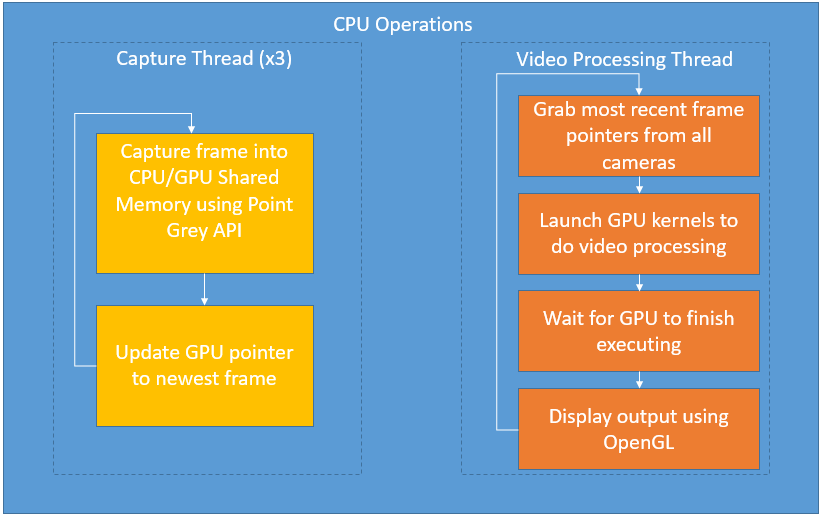
\includegraphics[width=0.6\textwidth,natwidth=610,natheight=642]{images/CPU.png} 
	\caption{CPU Operations: shows the functions of the different CPU threads}  
	\end{figure}
	
The GPU does all the heavy lifting in this program. It performs multiple video processing operations simultaneously. The GPU program is divided into several streams, each of which operates independently of the others, much like the multiple threads on a CPU. The Jetson allows multiple GPU kernels to run at the same time, as long as they are in different streams.
In the following diagram, each box represents a different GPU Kernel (with the exception of the bottom right box which is actually the same as the three bottom left kernels, just abbreviated to save space). These kernels are executed in order by their corresponding CUDA streams, which is essential. 
	
\begin{figure}[H] 
	\centering
	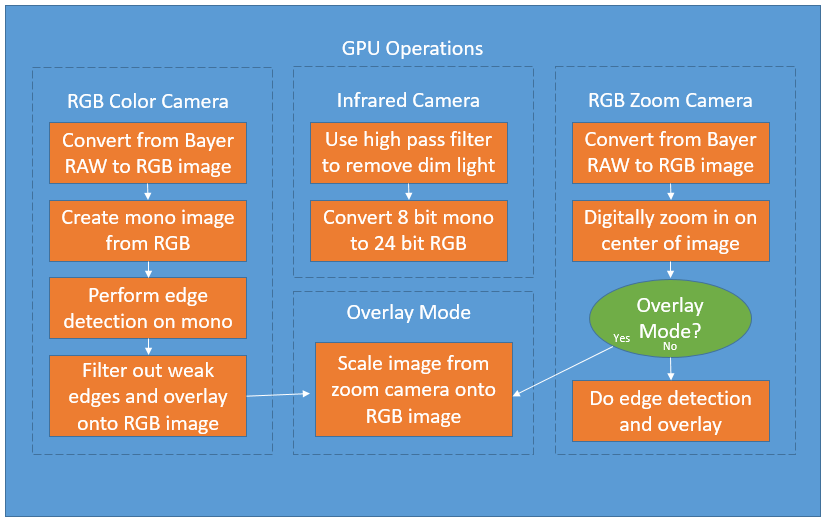
\includegraphics[width=0.6\textwidth,natwidth=610,natheight=642]{images/GPU.png}
	\caption{GPU Operations: shows the functions of the different CUDA streams}  
	\end{figure}
	
\subsection{Installation and Execution}
This software is designed to be a proof of concept that demonstrates the computing power of the NVIDIA Jetson TX1. It is not meant to be installed on other hardware, as it requires the use of the GPU present in the Jetson, and is specifically optimized to use the Jetson?s CPU/GPU shared memory that is not present on other devices. There are a number of example programs created using various filters and elements of the HawkEye system. They are run simply by executing them on the console.
\par
This software is designed specifically for the NVIDIA Jetson TX1 and for use with Point Grey USB 3.0 Cameras. It can be recompiled for other systems with CUDA-enabled GPUs however this has not been tested.

\subsection {Example Controls}
The example program we used at Expo has several controls.\\

Camera Views:
\begin{description}[leftmargin=2cm,labelindent=2cm]
	\item[\[1\]] RGB Camera
	\item[\[2\]] NIR Camera
	\item[\[3\]] Zoom Camera\\
\end{description}

Filters:
\begin{itemize}[leftmargin=2cm,labelindent=2cm]

\item RGB and Zoom Camera Views:
\begin{description}[leftmargin=2cm,labelindent=2cm]
	\item[\[G\]] Enable edge detection
	\item[\[F\]] Disable edge detection
	\item[\[H\]] Decrease edge detection threshold (more edges)
	\item[\[J\]] Increase edge detection threshold
	\item[\[\{\]] Zoom out
	\item[\[\}\]] Zoom in
\end{description}

\item RGB Only:
\begin{description}[leftmargin=2cm,labelindent=2cm]
	\item[\[Z\]] Enable zoom overlay
	\item[\[X\]] Disable zoon overlay
\end{description}

\item IR Only:
\begin{description}[leftmargin=2cm,labelindent=2cm]
	\item[\[G\]] Decrease IR Threshold (brighter image)
	\item[\[G\]] Increase IR Threshold (see only bright lights)\\
\end{description}

\end{itemize}

Quit Programs:
\begin{description}[leftmargin=2cm,labelindent=2cm]
	\item[\[Q\]] Quit
\end{description}

